\documentclass{beamer}

\usetheme{Copenhagen}

\makeatletter
\setbeamertemplate{headline}{}
\makeatother

\setbeamertemplate{footline}{}
\setbeamertemplate{page number in head/foot}[totalframenumber]
\setbeamertemplate{navigation symbols}{\footnotesize\usebeamertemplate{page number in head/foot}}

\usepackage[italian]{babel}
\usepackage[utf8]{inputenc}
\usepackage[T1]{fontenc}
\usepackage{pgfplots}
\usepackage{fdsymbol}
\usepackage{listings}
\lstset{
  language=Java,
  basicstyle=\tiny\ttfamily,
  keywordstyle=\color{blue}\bfseries,
  commentstyle=\color{green!60!black}\itshape,
  stringstyle=\color{orange},
  showstringspaces=false,
  breaklines=true,
  mathescape=true
}

\definecolor{color1}{HTML}{012A4A}
\definecolor{color2}{HTML}{013A63}
\definecolor{color3}{HTML}{01497C}
\definecolor{darkgreen}{HTML}{008000}

\setbeamercolor{palette primary}{bg=color1,fg=white}
\setbeamercolor{palette secondary}{bg=color2,fg=white}
\setbeamercolor{palette tertiary}{bg=color3,fg=white}
\setbeamercolor{block title}{bg=color2,fg=white}
\setbeamercolor{block body alerted}{bg=color2,fg=white}
\setbeamercolor{itemize item}{fg=color3}
\setbeamercolor{itemize subitem}{fg=color3}
\setbeamercolor{section in toc}{fg=color2}
\setbeamercolor{navigation symbols}{fg=color2}

\setbeamertemplate{section in toc}[circle]
\setbeamertemplate{itemize item}{\scriptsize$\vardiamondsuit$}
\setbeamertemplate{itemize subitem}{\scriptsize$\triangleright$}

\setbeamerfont{section number projected}{%
  family=\rmfamily,series=\bfseries,size=\normalsize}
\setbeamercolor{section number projected}{bg=color2,fg=white}


\title{\Large{Un classificatore di condizioni non soddisfacibili per migliorare l'efficienza di esecuzione simbolica}}

\author{\Large{Cristian Piacente} \\ \vspace{1.75mm} \small{Matricola 866020}}


\institute{{\textbf{{\color{color2}Relatore}}:
    \textit{Prof. Giovanni Denaro}\;\;\;\;\;
    \textbf{\color{color2}{Co-relatore}}: \textit{Prof. Pietro Braione}}\\
  \vspace{6mm}
  \small{Università degli Studi di Milano Bicocca\\Dipartimento di Informatica, Sistemistica e Comunicazione (DISCo)\\Corso di laurea in Informatica}}

\date[25/07/2023] {\footnotesize{Anno Accademico 2022-2023 \\ \vspace{3.5mm} 25 Luglio 2023}}

\logo{
\includegraphics[width=0.7cm]{img/logo.pdf}\vspace*{-0.4cm}\hspace*{\textwidth + 0.555555555}}

\setbeamertemplate{frametitle}
{
    \nointerlineskip
    \begin{beamercolorbox}[sep=0.3cm,ht=1.9em,wd=\paperwidth]{frametitle}
        \vbox{}\vskip-2ex%
        \strut\insertframetitle\strut
        \vskip-0.8ex%
    \end{beamercolorbox}
}

\pgfplotsset{compat=1.18}

\begin{document}

\setlength{\leftmargini}{0.5cm}

\begingroup
\setbeamertemplate{logo}{}
\setbeamertemplate{navigation symbols}{}
\begin{frame}[noframenumbering]
  \titlepage
\end{frame}
\endgroup


\begin{frame}{Contesto}
  \begin{itemize}
      \item Costruzione software di alta qualità $\Rightarrow$ testing
      \item Generazione automatica test $\Rightarrow$ riduzione costi, esplorazione spazio di input 
      \item Esecuzione simbolica: input $\Longleftrightarrow$ simboli
  \end{itemize}
  \begin{block}{Esecuzione simbolica dinamica}
    Combinazione di analisi statica e dinamica per la \textbf{generazione automatica di casi di test}
  \end{block}
\end{frame}

\begin{frame}{Obiettivo}
    \begin{alertblock}{}
    Massimizzare il numero di casi di test generati in un tempo limitato, evitando il tempo disperso per analizzare program-path non eseguibili
    \end{alertblock}
    \vspace{6mm}
    Per raggiungere l'obiettivo:
    \begin{itemize}
        \item adattamento del tool TARDIS
        \item machine learning
        \begin{itemize}
            \item viene integrata un'euristica per \textbf{classificare} le condizioni simboliche come soddisfacibili o non soddisfacibili
        \end{itemize}
    \end{itemize}
\end{frame}

\begin{frame}{Contenuti}
  \tableofcontents
\end{frame}

\section{Studio dell'esecuzione simbolica}
\begin{frame}[fragile]{Esecuzione simbolica dinamica (1/2)}
    \begin{block}{Concetti preliminari}
            Path condition, cammino feasible/infeasible, concolic execution
    \end{block}
    \begin{columns}[T]
        \begin{column}{0.77\textwidth}
            \vspace{-3mm}
            \hspace{1.5mm}
            \begin{minipage}{\dimexpr\textwidth-3mm}
                \begin{lstlisting}
public class MIPC {
  private final int[] a;
  private final int[] b;
  public MIPC(/* 15 int parameters */) {
    a = new int[]{a0, a1, a2, a3, a4};
    b = new int[]{b0, b1, b2, b3, b4, b5, b6, b7, b8, b9};
    for (int elemInB : b) {
      if (elemInB < 0) throw new RuntimeException();
    }
  }
  public boolean target() {
    int k = 0; boolean flag = true;
    for (int i = 0; i < a.length; ++i) {
      if (a[i] > 1000 + (1000 * i)) {
        for (int j = 0; j < b.length; ++j) {
          if (b[j] < -a[i]) { /* infeasible */
            k = 1;
          }
        }
      } else {
        flag = false;
      }
    }
    return (flag && k == 0);
  }
}
                \end{lstlisting}
            \end{minipage}
        \end{column}
        \begin{column}{0.22\textwidth}
        \vspace{5mm}
            \begingroup
            \setlength{\leftmargini}{-2mm}
            \begin{itemize}
                \setlength\itemsep{2em}
                \item Programma esempio particolare
            \end{itemize}
            \endgroup
        \end{column}
    \end{columns}
\end{frame}

% I know about the \only command but I prefer not to use it

\begin{frame}[fragile]{Esecuzione simbolica dinamica (2/2)}
    \begin{columns}[T]
        \begin{column}{\textwidth}
            \begingroup
            \setlength{\leftmargini}{13.3mm}
            \begin{itemize}
                \item \textbf{Generazione caso di test}
                \begin{lstlisting}
MIPC mipc = new MIPC(0, ..., 0);
boolean targetRes = mipc.target();
                \end{lstlisting}
                \setlength\itemsep{16.5pt}
                \item Calcolo path condition e PC alternative
                \begin{lstlisting}[breaklines=false]
A.length $\geq$ 0 && 0 < A.length && A[0] $\leq$ 1000 && 1 < A.length && 
 A[1] $\leq$ 2000 && 2 < A.length && A[2] $\leq$ 3000 && 3 < A.length && 
 A[3] $\leq$ 4000 && 4 < A.length && A[4] $\leq$ 5000 && 5 $\geq$ A.length
\end{lstlisting}
                \vspace{-0.8\baselineskip}
                \begin{itemize}
                \setlength\itemsep{-3pt}
    \item \lstinline|A == null|
    \item \lstinline|A.length $\geq$ 0 && 0 $\geq$ A.length|
    \item \lstinline|A.length $\geq$ 0 && 0 < A.length && A[0] > 1000|
    \item \lstinline|A.length $\geq$ 0 && 0 < A.length && A[0] $\leq$ 1000 && 1 $\geq$ A.length|
    \setlength{\itemsep}{-1.5pt}
    \item[] $\vdots$
    \item \begin{lstlisting}[breaklines=false]
A.length $\geq$ 0 && 0 < A.length && A[0] $\leq$ 1000 && 1 < A.length && 
 A[1] $\leq$ 2000 && 2 < A.length && A[2] $\leq$ 3000 && 3 < A.length && 
 A[3] $\leq$ 4000 && 4 < A.length && A[4] $\leq$ 5000 && 5 < A.length 
    \end{lstlisting}
                \end{itemize}
                \setlength\itemsep{0pt}
                \item Scelta path condition da passare ad EvoSuite
                \begin{itemize}
                    \item \textbf{Generazione caso di test} oppure timeout
                \end{itemize}
            \end{itemize}
            \endgroup
        \end{column}
        \begin{column}{0.53\textwidth}
            \vspace{-9.25mm}
            \hspace{-36.75mm}
            \begin{minipage}{\dimexpr\textwidth-3mm}
            \begin{lstlisting}[frame=single]
int k = 0; boolean flag = true;
for (int i = 0; i < a.length; ++i) {
  if (a[i] > 1000 + (1000 * i)) {
    for (int j = 0; j < b.length; ++j) {
      if (b[j] < -a[i]) k = 1;
    }
  } 
  else flag = false;
}
return (flag && k == 0);
            \end{lstlisting}
            \end{minipage}
        \end{column}
    \end{columns}
\end{frame}

\section{Analisi del problema di efficienza}
\begin{frame}{Cammini feasible}
    \begin{minipage}[c]{\linewidth}
        \hspace{-10.5mm}
        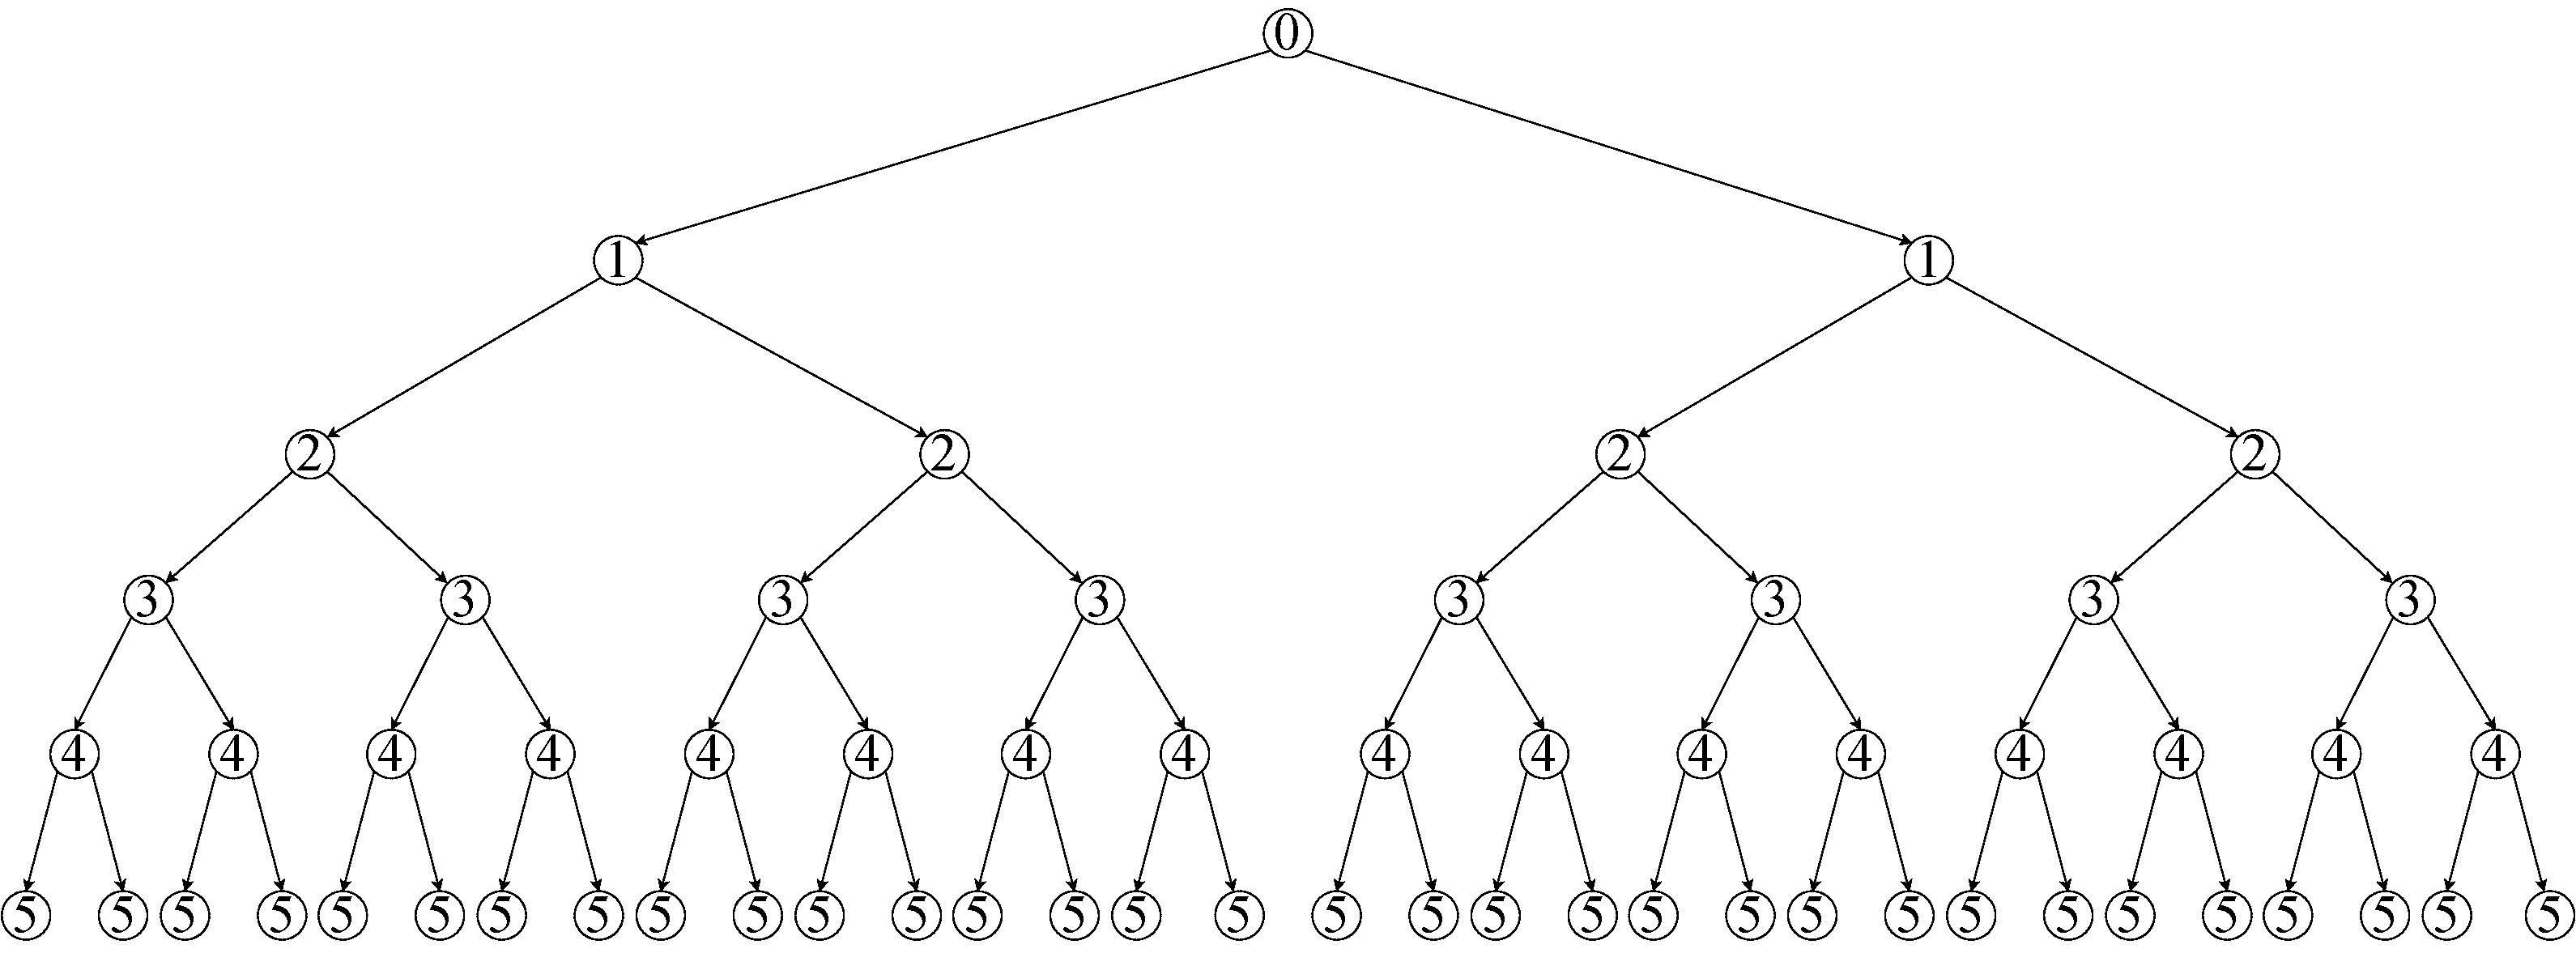
\includegraphics[width=12.72cm]{img/feasible-paths.pdf}
    \end{minipage}\\
    \vspace{6mm}
    \begin{minipage}[c]{\linewidth}
    \begin{columns}[T] % Align columns at the top
        \column{0.5\textwidth} % First column
        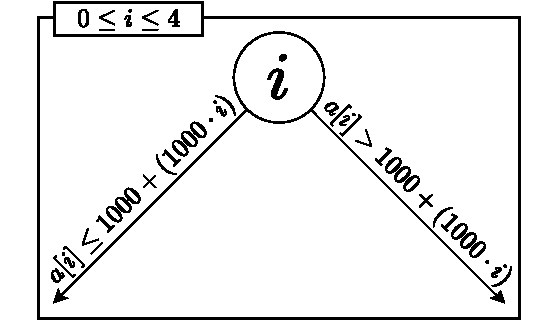
\includegraphics[width=\textwidth]{img/node-feasible.pdf}
        \column{0.5\textwidth} % Second column
        \begin{itemize}
            \item $2^5$ cammini feasible
            \item Centinaia di path condition non soddisfacibili
        \end{itemize}
        \vspace{-2mm}
        \begin{alertblock}{}
            Approccio: \textbf{classificare} le path condition alternative
        \end{alertblock}
    \end{columns}
    \end{minipage}
\end{frame}

\section{Progetto di classificatore}
\begin{frame}{Classificatore (1/2)}
    \vspace{-4pt}
    \begin{block}{Separazione in sottoformule}
        \begin{itemize}
        \item Chiusura transitiva \textbf{relazione di dipendenza} 
        \begin{itemize}
            \item infeasibility core
            \item contesto
        \end{itemize}
        \item Formule concrete e astratte
        \end{itemize}
    \end{block}
    \vspace{-4pt}
    \begin{block}{Struttura dati}
        3 \textbf{Bloom Filter}
    \end{block}
    \vspace{-4pt}
    \begin{block}{Classificazione ed estrazione probabilistica}
        \begin{itemize}
            \item \textbf{KNN} (K = 1)
            \begin{itemize}
                \item \underline{similarità} PC alternativa $\leftrightarrow$ training items
            \end{itemize}
            \item Code con diverse probabilità di estrazione
            \begin{itemize}
                \item PC unknown/feasible: \textbf{95\%}
                \item PC infeasible: 5\%
            \end{itemize}
        \end{itemize}
    \end{block}
\end{frame}

\begin{frame}{Classificatore (2/2)}
    \begin{minipage}[c]{\linewidth}
        \hspace{-11.28mm}
        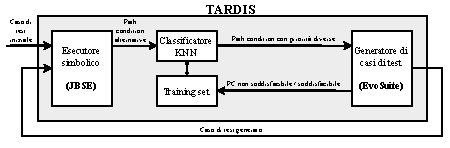
\includegraphics[width=1.195\textwidth]{img/tardis-diagram-classifier.pdf}
    \end{minipage}
\end{frame}

\section{Convalida su benchmark di 10 classi di programmi reali}
\begin{frame}{Risultati (1/2)}
    \begin{block}{Specifiche tecniche}
        OS Ubuntu 18.04.4 LTS 64-bit, 48 GB RAM (allocati 16 GB per esecuzione), CPU Intel Xeon(R) Gold 5120 @ 2.20GHz × 48 cores
    \end{block}
    \begin{block}{Benchmark}
        \begin{itemize}
            \item Parametri di configurazione
            \begin{itemize}
                \item 5 threads JBSE, 5 threads EvoSuite, 5 path condition alla volta, tempo globale \textbf{60 min}, tempo EvoSuite 7.5 minuti per processo
            \end{itemize}
            \item \textbf{10 classi} di progetti reali
            \begin{itemize}
                \item \textbf{6 esecuzioni} per ogni classe
                \begin{itemize}
                    \item 3 con il classificatore attivato
                    \item 3 senza l'uso del classificatore
                \end{itemize}
                \item numero max di test generati
            \end{itemize}
        \end{itemize}
    \end{block}
\end{frame}

\begin{frame}{Risultati (2/2)}
    \begin{figure}[h]
        \centering
        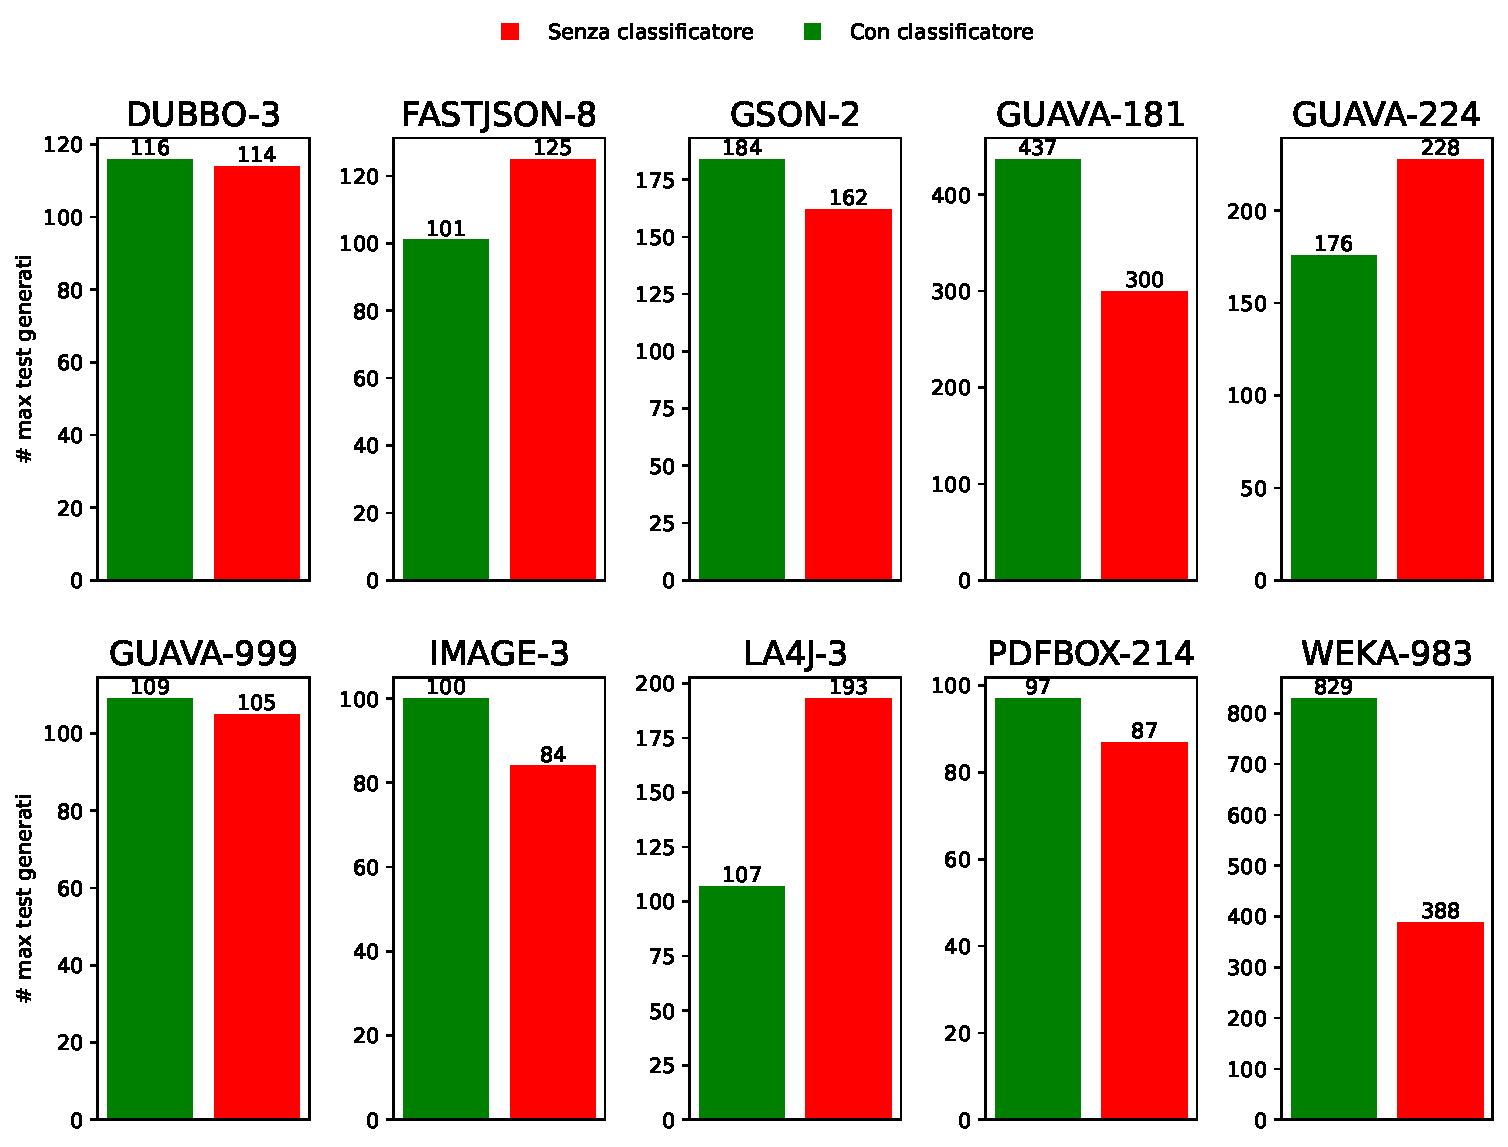
\includegraphics[width=\textwidth]{img/histograms-slide.pdf}
    \end{figure}
\end{frame}

\begin{frame}{Conclusioni}
    \begin{columns}[T]
        \begin{column}{0.5\textwidth}
            \vspace{-10mm}
            \begin{figure}[h]
                
\includegraphics[width=0.6\textwidth]{img/donut-chart.pdf}\\
                Miglioramenti
            \end{figure}
        \end{column}
        \begin{column}{0.5\textwidth}
                \begin{center}
                \vspace{-5mm}
                \begin{itemize}
                    \item Risultato migliore
                    \begin{itemize}
                        \item \textbf{\color{darkgreen}+441 test}
                    \end{itemize}
                    \item Risultato peggiore
                    \begin{itemize}
                        \item \textbf{\color{red}-86 test}
                    \end{itemize}
                \end{itemize}
                \end{center}
        \end{column}
    \end{columns}
    \vspace{5mm}
    \begin{block}{Sviluppi futuri}
        TARDIS attualmente risulta costoso in termini di risorse
        \begin{itemize}
            \item ottimizzazione spazio e tempo classi esistenti
            \begin{itemize}
                \item evitare che un numero elevato di clausole rallenti l'esecuzione simbolica (e.g. quando si controlla se una PC è ridondante)
            \end{itemize}
        \end{itemize}
    \end{block}
\end{frame}

\begingroup
\setbeamertemplate{logo}{}
\setbeamertemplate{navigation symbols}{}
\title{\Huge{{\underline{Grazie per l'attenzione!}}}}
\institute{}
\setbeamercolor{palette primary}{bg=white,fg=color3}
\begin{frame}[noframenumbering]
  \titlepage
\end{frame}
\endgroup


\end{document}